% the main points of this introduction are 
% outline the complexity of biological systems for physicists
% 	> even though our theoretical models should preidct everything on the energy and length scales of biology we can't because of their heterogeneity.
%   > Give examples of the heterogenaity 
% Give some points on the history of molecular biophysics  
%   >  Hodgkin-Huxley Models
%   > Gramicidin 
% Point out how Cystic Fibrosis is an expression of this progression, going from genotype to phenotype using an ion channel to teach us biophysics. 
% conclusion.
\chapter{A Physical Introduction to Theoretical Biology}
\pagenumbering{arabic}
\setcounter{page}{1}
\label{chap:introduction}
%\chapquote{Whatever complexity means, most people agree that biological systems have it.} {Frauenfelder and Wolynes \cite{frauenfelder1994}}

\begin{chapquote}  {Frauenfelder and Wolynes \cite{frauenfelder1994}}
Whatever ``complexity" means, most people agree that biological systems have it.
\end{chapquote}

%\vspace
\section{Thesis and Chapter Summary}

This thesis seeks to apply a philosophy of molecular biophysics, to demonstrate its capability to investigate pressing problems in biology and medicine. In particular, we will use molecular dynamics (MD) to look at how a specific gene misfunctions to cause disease. The disease in question is Cystic Fibrosis (CF), and it is caused by the misfunction of a protein called the Cystic Fibrosis Transmembrane Conductance Regulator (CFTR). These MD techniques will allow us to formulate a model of CFTR's misfunction which we hope will direct research efforts and allow more patients suffering from CF to access life saving medication. 

In this first short chapter we will quickly build a philosophy which outlines how to look at biology through the lens of a physicist. To do this we will first outline what the goal of a physicist is: to create abstract formalisms which can be used to model the natural world. We will then observe what makes the construction of such formalisms so difficult for biological problems. 

These difficulties have often led biophysicists to study ion channels. Because of their simplicity, and their importance to cellular function, these molecules have served as laboratories to understand more complex biological systems, such as whole cells or organisms. 

Chapter \ref{chap:methods} will describe the chemical and numerical simulation techniques we have used to study the CFTR protein system in detail, while chapter \ref{chap:cftr} gives an overview of the CFTR system itself, and also a set of \textit {in vitro} assays which compliment our computational modelling.  Chapters \ref{chap:I37R}, \ref{chap:R352Q}, \ref{chap:S945L} and \ref{chap:opening} demonstrate the details of how a diverse application of the simulation techniques in chapter \ref{chap:methods} can be used to discover the unique modes of misfunction in CFTR. In combination with \textit {in vitro} cellular techniques, these simulation results prove that these existing drug regimens can rescue many molecular defects. Finally, chapter \ref{chap:perspective} ties together these results to argue for a physical model which elucidates the mechanism of action for cystic fibrosis drugs. Armed with this model we will work through the available literature and identify some priorities for future studies using molecular modelling for cystic fibrosis research. 

%In chapters \ref{chap:methods}, \ref{chap:cftr} and \ref{chap:perspective} considerable care has been taken to give an overview of the many aspects of computational methods using MD and the cellular, molecular and clinical research into CF to give future readers a detailed reference text should they too wish to study CF.

We hope this small example can demonstrate the utility of physics expertise for the field of molecular medicine. We anticipate that such methods will only grow in power with improvements in computational and experimental techniques.

\section{What is Physics?}
\label{WIP}
Before I started university I described physics as ``the study of how things move". Although intuitive, this description does not shed light on the philosophy of doing physics which make it such a powerful tool for understanding the natural world. When we create a predictive physical theory, we first carefully define a formalism motivated by patterns we see in the world around us. Then, using mathematics, the implications of this formalism are built up to make predictions about measurable phenomena. Should the predictions from the formalism agree with experimental results, it validates the formalism, giving rise to a physical theory. This is what makes physics feel like the most ``fundamental" of the natural sciences.

%\footnote{The natural sciences include chemistry, biology, physics.  Mathematics and logic are forms of the formal sciences, which we rely on heavily as natural scientists. }

These formalisms make use of many mathematical objects. Examples you might be familiar with include:
\begin{itemize}
\item The gas of hard spheres, which we use to derive the Boltzmann's kinetic theory of gasses.  
\begin{equation}
	\label{hard_spheres}
	\frac{\partial f_1}{\partial t} + \frac{\bold{F}}{m}\cdot\nabla_\bold{r} + \bold{v} \cdot \nabla_\bold{r} f_1 =  \int \int (f'_1f'_2 - f_1 f_2) \tilde \kappa d \hat \kappa d \bold{v}_2.
\end{equation}

\item The interacting electric and magnetic vector fields in Maxwell's laws of electromagnetism \cite{griffiths2017}.
\begin{equation}
	\begin{aligned}
	%\nabla \dot \mathbf{E} = \frac{\rho}{\epsilon_0}
		\nabla \cdot  \mathbf{E} &= \frac{\rho}{\epsilon_0} \qquad & \nabla \cdot  \mathbf{B} &= 0 \\
		\nabla \times  \mathbf{E} &= -\frac{\partial \mathbf{B}}{\partial t} \qquad &  \nabla \cdot  \mathbf{B} &= \mu_0 \big(\mathbf{J} + \epsilon_0 \frac{\partial \mathbf{E} } {\partial t }\big).
	\end{aligned}
\end{equation}

%\partial_\alpha F^{\alpha \beta} = \frac{4\pi}{c} J^\beta
\item The Riemannian manifolds which define the curvature of spacetime in Einstein's theories of relativity \cite{carroll2019}.
\begin{equation}
	G_{\mu \nu} + \Lambda g_{\mu \nu} = \kappa T_{\mu \nu}.
\end{equation}

\item The complex probability waves which evolve according to Schr\"oedinger's equation, describing quantum mechanics \cite{griffiths1994}. 

\begin{equation}
	i \hbar \frac{d}{dt} | \psi (t) \rangle = \hat {H} | \psi (t) \rangle .
\end{equation}
\end{itemize}

As biophysicists we would wish to find the most basic formalisms for biological phenomenon, so we can fully understand the function of an organism. The quest for such a formalism has an interesting origin. In 1944 Erwin Schr\"oedinger wrote an essay titled ``What is Life?" This remarkable work was written before the discovery of DNA's structure or the maturation of information theory. Schr\"oedinger used first principles in thermodynamics and quantum mechanics to speculate at the nature of life at the atomic level. The most remarkable thing about this essay is how much the author got right. 

He observed that since organisms exist at temperatures on the order of 300 Kelvin, the physical encoding of genetic information inside cells must be chemical in nature---since at such temperatures the physical arrangements of atoms would be unstable without chemical bonds. By estimating the amount of information that could be stored in an arrangement of atoms, Schr\"oedinger posits the existence of what he calls an ''aperiodic crystal". Although not a crystal in the rigorous sense, the double helix structure of DNA is not far from such an analogy. As Figure \ref{dna_structure} shows, the DNA double helix is a combination of periodic and aperiodic elements, not too different from how one might visualise a one-dimensional aperiodic crystal \cite{varn2016}. This allegory is an example of how physical principals can be used to direct questions in fundamental biology. In fact, James Watson credited Schro\"edinger's book as one of his influences in how he visualised the structure of the DNA before its discovery through X-ray crystallography \cite{watson2010}.

\begin{figure}
	\begin{center}
		
\includegraphics[width=1.0\textwidth]{figures/dna_backbone_aperiodic_crystal.pdf}
	\end{center}
	\captionsetup{singlelinecheck = false, justification=raggedright}
	\caption[The Structure of DNA has Periodic and Aperiodic Elements] {\textbf{The Structure of DNA has Periodic and Aperiodic Elements}}{Although not a crystal, the structure of DNA has some periodic and some aperiodic elements. This is reminiscient of Schr\"oedinger's speculation that genetic information is chemically encoded in an aperiodic crystal. }
	\label{dna_structure}
\end{figure}

In this example, Schr\"oedinger naturally chose a formalism of interacting atoms, mostly consistent with the statistical mechanics in equation \ref{hard_spheres}, to arrive at his model of an aperiodic crystal. In this thesis we will use a more careful, but similar formalism to study the function of the CFTR protein. We will outline this formalism in detail in chapter \ref{chap:methods}. The goal of chapters \ref{chap:cftr}-\ref{chap:opening} is then to collect evidence in order to develop a physics inspired model of for the treatment of Cystic Fibrosis disease, which we will propose in chapter \ref{chap:perspective}. The model we arrive at is more abstract than physicists are used to, and the next section will explore why this is often the case for biological systems.
 
%Somewhere on the scale between a single protein and a single cell this is what we consider "life". We have single unicellular organisms but we don't have uniproteomic organisms. So the fundamental length scale of life is somewhere between $10^{-10}m$ and $10^{-3}m$. This is the first loop in our strange loop.

%Biological strange loops would not seem to be as self similar as the clean nice logics in the strange loop of the Godelian knot. Why is this?

\section{The Physics Inside your Cells}
%purpose of this section is to 

Why can't I write down an equation which will tell me how long I will live? Or how tall I will grow?

These might seem like odd questions but if you asked a physicist how much power it would take to ionise a gas or how long it will take a black hole to evaporate itself out of existence, they would have a tool kit of highly accurate models to help them calculate solutions. 

To understand why the first set of problems are so much more difficult for physicists, we will analyse the cases where physics fails. Any physical theory may fail for one of the following three reasons: 

\begin{itemize} 
	\item The physicist does not have sufficient computational power to integrate the formalisms in the relevant theory, so they cannot make predictions about a specific phenomenon.

		\item The physicist lacks sufficient data, so they cannot specify reasonable initial conditions for the calculations with the formalism. 

		\item The phenomenon in question lies outside the applicable energy or length of the physical theory.This would occur, for example, if we used Newton's theories of gravity to predict the motion of an object around a super-massive black hole---here we would instead need Einstein's general theories of relativity \cite{picker2022}.

\end{itemize}

From the perspective of fundamental physics, quantitative theories of biology fail for one of the first two reasons. Given the energy and length scale of biological systems, we currently possess the necessary theoretical tools to simulate every interaction inside a living being \cite{carroll2021}. 

The difficulty of studying biology then, does not arise from a lack of physical understanding. As we will see in chapter \ref{chap:methods} the physics of the molecular interactions in living things is surprisingly simple. Rather, the difficulty of biological problems arises from the sheer number of interactions we must consider. Inside cells we find proteins, lipids, solvents, salts each with their own physical properties. Therefore, biophysics distinguishes itself from more traditional physics by considering systems that are both highly heterogeneous and anisotropic. This aspect of biological systems makes it difficult to scale up our formalisms to make predictions using human tractable mathematical tools---meanwhile, computational engines can only help so much. Hence, we have to be careful about which systems we study with our available toolkit. When their computational or theoretical tools were lacking, physicists often turned to ion channels as laboratories to develop and test biophysical theories \cite{moy2000, corry2000}.

%For biological systems there appears to be too much complexity for such analogies to have the same level of success. 

%Although considerable success can be found in modelling biology with formalisms that do not stem directly from fundamental physics, such models must be tailor made in order to treat specific phenomenon \cite{phillips2012}. The advantage of MD and the formalism of interacting atoms in chapter \ref{chap:methods} is that they are the most accurate available to the biophysicist. The issue is the considerable computational load attached to them. 

%Thus, in order to move towards more predictive theories of biology it is necessary to develop layers of physical theories applicable in different contexts. One form of this from fundamentals approach is the simulation of every atom in a biological system. Although computationally expensive, this approach has been proven necessary when studying the molecular details of proteins, due to the heterogeneous nature of biological systems . 


%One of the things we're trying to do with molecular dynamics is fill in the gap left by the sequence->function paradigm which is internalised in current understandings of molecular biology. We usually talk about how the sequence of the gene defines its function because it gives the protein its structure but really there is a considerably larger amount of regulatory pressure exerted by the environment. This is what is missing from the sequence alone paradigm.

%Biological systems exhibit such a problem for the physicist because unlike the above problems it is extremely hard to pick out a fundamental unit to even begin our upwards journey. An evolutionary biologist might say to choose the "gene" but this is actually far too high in our spatial heirarchy already. Really, a gene is only meaningful to the dance of life if it has partners to dance with. 

%A coil of DNA in water doesn't really do much in solution except decay without machinery that can preserve, read, translate and replicate it. The gene is an emergent property, we have to go deeper. 

%So, what are the gene's partners? 

%A slew of biological machinery that mostly take the form of proteins. These proteins are a special case of chemistry, with many observable functions. Their sequence is  coded by the DNA in something reminiscent of a strange loop \cite{hofstadter2007}. 

%This self referential loop is one of the reasons biology is so difficult. Since we know that this strange loop is kicked off by atomic interactions we will start there. As we are taking a physical, pragmatic approach here it would make sense to begin with the protein, after all, they stave off the march of entropy constantly trying to eat up all of your cells. It also just so happens that they are much easier to understand computationally since their motions are faster and more flexible. 

%The first level sub cellular organisation is perhaps the most intimdating first step for me personally after spending 4 years simulating a single protein. Glimpsing the complexity within a single one of these molecules has been one of the most existential experiences of my life but the knowledge that there are astronomical numbers of these things inside me all of the time terrifies me.

%It is hoped that illustrating the monumental amount of both intellectual effort and material resources of incrementally increasing the understanding of a single protein amongst the 23000 or so encoded in our genome will give the reader and understanding of how we might continue our quest to understand the molecular dance that plays within all of us.

%After this things start to run away from me with my handful of GPUs and limited patience. So in this thesis we will only discuss single proteins.

\section{Using Ion Channels as Natural Laboratories to Study Biophysics}
\label{ion_channel_laboratories}

Ion channels are a special kind of protein which allow the passage of charged particles to pass across the membrane of a cell. They are excellent laboratories for the study of biophysics for two reasons. Firstly, it is very easy to measure their activity with a technique called electrophysiology which we will briefly explore in chapter \ref{chap:cftr} \cite{hille2001}. Secondly, they are critical to the health and function of cells. As cell biology has advanced, it has become increasingly clear that the level of polarisation (potential difference from the inside to the outside) in a cell is critical to its function. Cell polarisation regulates many chemical reactions \cite{catterall2011, muthuswamy2012, levin2014, levin2014a}.\footnote{A back of the envelope calculation reveals that a -100mV resting potential is a 2.5 kcal/mol barrier to the transport of molecular species with a charge of -1e into the cell. This is not an insignificant energy contribution.} 

It is perhaps then not surprising but nonetheless remarkable that ion channels are the targets of 19\% of clinically approved drugs \cite{santos2017}. However, there is much more work to be done, as candidate drugs are often insufficiently selective for the desired ion channel, leading to sometimes lethal side effects \cite{stansfeld2006, kaczorowski2008, waszkielewicz2013}.

Historically, ion channels have served as a testing ground for biophysical models. The first interest in modelling their behaviour comes from the experiments of two biophysicists, Andrew Hodgkin and Alan Huxley. They threaded silver wires through the thick nerves of a giant squid and measured the current running through the nerve in response to electrical stimulation. What they found was intriguing. Signals would only propagate down the nerve when the input signal was of a sufficient high voltage. They managed to match their experimental data with a model comprised of the following set of ordinary differential equations:

\begin{equation}
	\label{hh_equations}
\begin{aligned}
	I = C_m \frac{dV}{dt} + \bar{g}_K& n^4 (V - V_K) + \bar{g}_{Na} m^3 h (V - V_{Na} ) + \bar{g}_l (V-V_l) , \\ \\
	\frac{dn}{dt} &= \alpha_n(V)  (1-n) - \beta_n(V)  n, \\ \\
	\frac{dm}{dt} &= \alpha_m(V)  (1-m) - \beta_m(V)  m, \\ \\
	\frac{dh}{dt} &= \alpha_h(V)  (1-h) - \beta_h(V)  h.  
\end{aligned}
\end{equation}

Here, the $n,\ m$ and $h \in [0,1]$ parameters are associated with potassium channel subunit activation, sodium channel subunit activation, and sodium channel subunit inactivation, respectively. $C_m$ is the capacitance of the lipid membrane per unit area, and $\bar{g}_i$ is the maximal conductance allowed across the membrane, per unit area. The terms $V_i$ denote either the total voltage, or the contribution to the total from a specific charged species. 

The solutions to the Hodgkin-Huxley model allow us to mathematically discover and describe several important cellular functions. The model encodes both the existence of a cell's resting potential and the behaviour of selective voltage-gated ion channels. Even today, the molecular mechanisms behind these discoveries are used to understand protein and cellular function \cite{aidley1996}. This curve created by the action potential is a common sight in many physiology textbooks, and it is in fact a solution to this coupled set off ODES \cite{pollard2016}.

\begin{figure}
	\begin{center}
		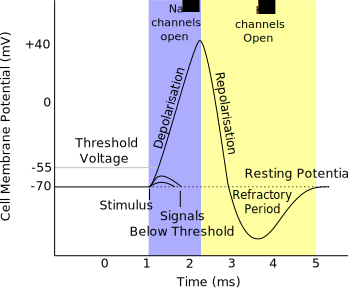
\includegraphics[width=0.9\textwidth]{figures/Hodgkin-Huxley_action_potential.pdf}
	\end{center}
	\captionsetup{singlelinecheck = false, justification=raggedright}
	\caption[The Action Potential is a Solution to the Hodkin-Huxley Model] {\textbf{The Action Potential is a Solution to the Hodgkin-Huxley Model }}{ A) The ``voltage clamp" experimental set up which was used to study nerve impulses \cite{hodgkin_huxley_figure_website}. A giant squid nerve was submerged in sea water and an electrode was threaded through it as shown. The voltage was recorded as impulses were fired into the nerve. B) The shape of the action potential is a familiar sight in many physiology textbooks. The physical basis for its shape was realised through the mathematical modelling of Hodgkin and Huxley which won them the 1963 Noble Prize in physiology or medicine. This discovery is an example of the physiological importance of ion channels and also how deep theoretical insight can lead to predictive models of living systems \cite{hodgkin1952, hodgkin1952a, hodgkin1952b, hodgkin1952c, hodgkin1952d}.}
	\label{action_potential_graphic}
\end{figure}

The equations in the model \href{hh_equations}{above} are an example of the development of a mathematical formalism which is not fundamental in the same way as the equations at the beginning of section \ref{WIP}. But rather, the model above is built for an express purpose: to predict and describe the propagation of signals through a nerve. This model shows how quantitative thinking can lead to insights in biology. The sheer complexity of biology demands this of us. We cannot create complete theories so we must find useful formalisms for small domains of the problem space.

\begin{figure}
	\begin{center}
		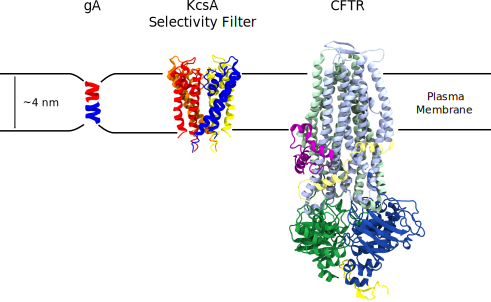
\includegraphics[width=0.8\textwidth]{figures/ion_channel_progression.pdf}
	\end{center}
	\captionsetup{singlelinecheck = false, justification=raggedright}
	\caption[Different Ion Channels Amenable to Molecular Simulation] {\textbf{Different Ion Channels Amenable to Molecular Simulation}}{Gramicidin A was initially used as a toy model to test different \textit{in silico} modelling techniques (PDB ID 1NT5) \cite{sham2003}. KcsA, is a bacterial potassium channel. This structure only comprises the pore domain, also called the selectivity filter (PDB ID 1BL8) \cite{doyle1998}. This structure drew interest because potassium channels play an important role in the function of cells. Finally, the CFTR anion channel about which this thesis is written (PDB ID 6MSM) \cite{zhang2018a}. In the course of 30 years we have gone from simulating just a few nanoseconds of Gramicidin A to collecting almost half a millisecond of data for this thesis by simulating the much larger CFTR. This heralds an exciting future for computational biophysics \cite{roux1993}. What is even more exciting will be the next 30 years. At the time of writing, a computational engine named Anton 3 has come online. This purpose built computer could perform all the calculations in this thesis in less than a week \cite{jones2022, russell2021}. That's not a week in parallel, that's in serial!}
	\label{ion_channel_progress}
\end{figure}

In this thesis we aim to do something similar. By building up from the fundamental physics outlined in chapter \ref{chap:methods}, we will build a model for the dysfunction of a single gene (CFTR), to understand a disease (CF). Again, we do not possess sufficient computational power to produce a complete physical model of CF, so we will have to settle for a qualitative model, which we will outline in chapter \ref{chap:perspective}. 

%The measurements and modelling they carried out gave an exciting set of results. They found that the cell had to maintain a constant voltage gradient, they discovered that the presence of voltage gated ion channels and cation selective ion channels \cite{hodgkin1952}. Each of these features, motivated by mathematical modelling have been found to be critical to the functioning of the cell and fundamental to the foundation of molecular biophysics.    

\subsubsection{Computer Modelling the Dynamics of Ion Channels}
Motivated by the advances in cell biology that arose from the Hodgkin-Huxley model, early adopters of computational biophysics such as Martin Karplus, Beno\^it Roux, Klaus Schulten, J. Andrew McCammon, Shin-Ho Chung, Mark Sansom, Helmut Grubm\"uller, Serdar Kuyucak and Toby Allen devoted significant parts of their career to studying ion channels \cite{mccammon1977, sansom1991, roux1991, roux1993, sansom1991, tajkhorshid2002, degroot2001, allen2003, allen2004, chung2002, tieleman2001}. 

These early studies usually focussed on gramicidin A (gA) because of its small size, its amenability to structural characterisation and the opportunity to compare experimental measurements with \textit{in silico} calculations \cite{urry1971,arseniev1985,wallace1986,wallace1998}. This small antibacterial peptide assembles into a coil which selectively allows the passage of potassium ions in the cell walls of gram-positive bacteria. This bleeds dry the bacteria's internal potassium concentration, which is critical to cellular function \cite{liou2015}. For a long time, gA was the only protein ion channel with its structure determined to atomic resolution. Because ion channels are membrane proteins, it took further advancements in experimental structural biology techniques by Roderick Mackinnon and others to determine the atomistic structures of other channels \cite{kuhlbrandt2014, clapham2003, doyle1998}. 


The careful work on gA enabled the development of theoretical and computational methods which can now be transferred to the more biologically important channels, such as potassium and sodium ion channels \cite{rashid2013, li2021, vandenberg2021,flood2019}. With the ``resolution revolution" in structural biology, driven by the maturation of cryo-EM structural biology and even more recently AI based structure predictions, we are entering an era of structural abundance---there are now literally thousands of biologically relevant targets which we can study with simulations \cite{jumper2021, frank2021, cheng2017a}. 

%This careful work on gA aided the development of many computational techniques. Along with an abundance of protein structures and other experimental advances, of this kind of modelling and experimental techniques the molecular details of the function of ion channels has become accessible to computational techniques \cite{flood2019}. The careful work on gA enabled the development of theoretical and computational methods which could then be transferred to the more biologically important channels such as potassium channels once they were structurally characterised by the laboratories of Roderick MacKinnon and others \cite{rashid2013, li2021, vandenberg2021}. Now with the ``resolution revolution" occurring in structural biology with the maturation of cryo-EM structural biology and now AI based protein predictions we are entering an era of structural abundance. 

In this new era, ion channels will likely continue to be important clinical and biophysical targets. In addition to the propagation of nerve signals we saw in section \ref{ion_channel_laboratories}, they play a critical role in all 5 senses, allowing cells to react to pressure (and hence touch) \cite{chesler2018}, temperature \cite{castillo2018}, pain \cite{kingwell2019}, acids \cite{kweon2013} and smell (in insects) \cite{sato2008}. There is also an exciting subfield emerging which investigates the role of ion channels in the bioelectrical networks which regulate cell morphogenesis and growth \cite{lang2005, sundelacruz2009, levin2014, levin2014a}.

As we have shown, the historical goal of computational biophysicists has been to use whatever physical models and structural information is available, to understand living things at the molecular level (Figure \ref{ion_channel_progress}) \cite{lev2020, chen2021}. In this thesis, we seek to continue this trend, by applying the fundamental physical models described in chapter \ref{chap:methods} to study a disease, Cystic Fibrosis, at the molecular level.

%The availability of protein structures and the maturation of computational methods has enabled diverse studies of ion channels and other protein systems . Some of this progress has been summarised in figure \ref{ion_channel_progress}. In this thesis we have continued this trend, by applying the theoretical and computational techniques to study an ion channel and toward develop a theoretical model which helps us study a disease, Cystic Fibrosis. 

\section{Studying Cystic Fibrosis; Toward a Molecular Theory of Disease.} 

The sad truth of Cystic Fibrosis (CF) is that those afflicted are extremely unlucky. A small change to their genome causes their lungs to fill with sticky mucus and become infected with bacteria---each breath becomes cumbersome \cite{katkin2022}. Historically, diseases have been diagnosed based on symptoms and not causes \cite{foucault1994}. As section \ref{WIP} outlines, this is antithetical to how we would like to study a physical process, even a biological one. 

To build a predictive model, we would like to understand the root cause of a disease so we can predict how to treat it. Discovering this root cause can be extremely difficult and often requires decades of clinical enquiry \cite{dubois2016, tsui2013}. CF has the helpful characteristic of being a monogenic disease, so our molecular theory of this disease can begin by considering a single protein system and then slowly build outward, to  consider other genes which effect the disease as well.

In this way, my motivations for studying the CFTR protein are not solely focussed on treating disease. This problem is also an interesting opportunity to develop molecular theories of biology. This is what motivated the basic biophysical studies in chapter \ref{chap:opening}. 

When understanding CFTR, a helpful perspective can be gained from the following model of protein evolution. It states that the stability of a protein's structure contributes to the overall fitness of an organism by a formula \cite{depristo2005}:

\begin{equation}
	\label{fitness_equation}
	W(\Delta G) \propto \exp\bigg(\bigg[-\frac{\Delta G - \Delta G_{opt}}{\sigma_{\Delta G}}\bigg]^4\bigg) + c.
\end{equation}

Here, $W$ represents the evolutionary fitness of an organism, $\Delta G$ is the folding energy of the protein with a given gene sequence and $\Delta G_{opt}$ is the folding energy of the protein in the average (fit) population. The parameter $\sigma_{\Delta G}$ controls how broad this distribution will be and depends significantly on the protein physics of the gene. Figure \ref{fitness_landscape_figure} demonstrates the types of random walks a gene might take through sequence space, according to this model. 

There are over 400 recorded mutations which cause CF \cite{cftr2}. This indicates that  the CFTR gene exhibits an exceptionally small $\sigma_{\Delta G}$, so the band in the modified gaussian in figure \ref{fitness_landscape_figure}a is very narrow. This means that CFTR sits at the precipice of a daunting cliff in sequence space.  So, by taking small steps in sequence space and figuring out what factors have caused $W$ to decrease, we can try to understand how we might push the needle of protein stability back into the optimal zone. Once we understand how we can do this for CFTR, we can use such thinking to build our methods outward and apply it to other diseases, such as sickle cell anemia, Alzheimer's disease, and Huntington's disease \cite{depristo2005}.

	\begin{center}
		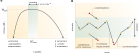
\includegraphics[width=1.0\textwidth]{figures/fitness_landscape_fig.pdf}
	\end{center}
	\begingroup
	\captionsetup{singlelinecheck = false, justification=raggedright}
	\captionof{figure}[A Physical Model to Understand Protein Evolution] {\textbf{A Physical Model to Understand Protein Evolution}}{a) The stability of a protein can be measured by its folding free energy $\Delta G$. This is related to the fitness of an organism $W$ by equation \ref{fitness_equation}. This model gives rise to a peaked distribution which helps us understand how so many mutants can give rise to cystic fibrosis. It appears as though the CFTR gene has an exceptionally narrow $\sigma_{\Delta G}$ and so small changes to the sequence of the gene have a comparatively dramatic effect on the evolutionary fitness of the organism. b) The model in equation \ref{fitness_equation} gives rise to a random walk through sequence space for subsequent generations. In the case of CF, it would appear as though \textit{homo sapiens} are stuck at a specific snapshot in evolutionary time where CFTR may easily lose function. So, without gene therapies which can modify a gene sequence \textit {in vivo}, we must use small molecule drugs and other medical interventions to somehow broaden the peak in equation \ref{fitness_equation}.}
	\label{fitness_landscape_figure}
\endgroup

CF is an excellent disease with which to begin such a project. Due to the array of disease causing mutations which occur across the CFTR protein, there is a large body of literature on its unique function \cite{csanady2019a}. This presents the opportunity to simultaneously perform basic biophysical research, while directly assisting in the improvement of patient outcomes. This is the sort of inquiry which drives basic science forward---combining interesting experimental data into theoretical models to make testable predictions. The aim of this thesis is to build a model to help direct efforts which will hopefully produce better patient outcomes. In chapter \ref{chap:perspective}, we will combine evidence from the existing literature with our biochemical and simulation results to build our predictive model. It is hoped that this model can help direct future strategies to treat CF.

%As we will see in chapter \ref{chap:cftr}, the integration of basic biological research into the treatment of disease can drastically improve patient outcomes. In this particular context, we have studied a single gene. But eventually, similar thinking will be able to build out our understanding consider multiple genes in as much detail, giving us a more complete picture of both life and disease, heralding the exciting future for biophysics. 

\section{The Future is Biological}
Biological sciences have important applications in medicine, agriculture and increasingly, manufacturing \cite{anonymous2019, scown2022}. We are in the midst of developing biology from a descriptive, to a predictive science \cite{kochanski1973,liu2005, mogilner2016, covert2021, jumper2021}. This transition is being driven by the combination of refined experimental techniques, rich datasets, strong theories and powerful computational engines. This is exciting because biological systems have happened upon ingenious solutions to some very difficult problems with the help evolution \cite{dawkins1989, dawkins2016}. Evolution has done much of the hard work for us, and as we understand it better, we can begin to apply its solutions to our own problems \cite{benyus2009, wang2021a, arnold2018}.

Throughout science, the integration of experimental data with theoretical models leads to new discoveries. In the case of biology, wet lab scientists take advantage of experimental techniques which allow them to understand the structure and dynamics of living things from the top down. The finer the experimental instrument, the finer the detail they may resolve. Conversely, computational and theoretical biologists take a bottom up approach. Like physicists, they aim to take the granular details of a system and integrate them upwards, to model and predict the macroscopic behaviour of a system. 

With more powerful computers and more detailed theoretical models, theorists can make predictions about the behaviour of more complex systems. What is so exciting about the current era of biological research is that the domains of these two approaches are beginning to overlap, where they can synergize and drive further breakthroughs \cite{anonymous2019}.

This has been happening in physics for decades, resulting in world changing breakthroughs like telecommunications, nuclear power and transistors \cite{wu2009}. The reason this has been possible for physicists is that the systems they usually study are homogeneous. They include just a few, albeit sometimes complex components. Hence, it is much easier to integrate a theoretical formalism upward and predict measurable phenomenon. 

The difference with biological systems is that they have so many different components. Hence, finding an analytic or even computationally tractable solution is usually impossible. However, as we collect more data with increasingly advanced experimental techniques\footnote{Important biophysical techniques one will encounter often in the literature are cryogenic electron microscopy (Cryo-EM) \cite{cheng2015, callaway2015, callaway2020}, electrophysiology \cite{aidley1996}, nuclear magnetic resonance (NMR) spectroscopy \cite{marion2013}, confocal and fluorescence microscopy \cite{sanderson2014}, X-ray Crystallography \cite{frauenfelder2010, drenth2006}, and genetic engineering (explanations of CRISPR-Cas9 or inverse PCR based techniques can be found in \cite{silva2017} and \cite{crispr2019}, respectively)} and build more powerful computers, more biological problems will become tractable. These, in turn, inform more detailed theoretical techniques which help direct the material efforts of experimental studies. 

\subsubsection{Onward and Upward}

This introductory chapter has given us an overview of the philosophy behind physical biology, how we intend to apply it to study CF, and the exciting advances we can expect from future developments in biophysics. It is this same structure that we will use throughout the thesis. Chapter \ref{chap:methods} will use our philosophy of physics to take a formalism of interacting atoms and integrate it upward to model biomolecular systems. We will then collect a large number of molecular details about the molecular cause and treatment of CF in chapter \ref{chap:cftr}. This will give us the starting starting point for our own contributions to the study of CF in chapters \ref{chap:I37R}, \ref{chap:R352Q}, \ref{chap:S945L} and \ref{chap:opening}. These results will allow us to collect evidence to help formulate the molecular model in chapter \ref{chap:perspective} to understand the treatment of CF. With this roadmap, we will now begin our journey upward in chapter \ref{chap:methods}, by diving deep into the molecular dynamics methods which will allow us to model the molecular basis of Cystic Fibrosis.

%Armed with this philosophy we will delineate how to use the formal object of the Schr\"oedinger wave equation to make approximations to atomic systems in order to create a biophysical model for macromolecular systems like proteins.
